%%%%%%%%%%%%%%%%%%%%%%%%%%%%%%%%%%%%%%%%%%%%%%%%%%%%%%%%%%%%%%%%%%%%%%%%%%%%
%                                                                          %
%      This file is part of the 'musicexamples' LaTeX package.             %
%                                =============                             %
%                                                                          %
%              https://github.com/uliska/lilyglyphs                        %
%                                                                          %
%  Copyright 2012-2014, 2018 by Urs Liska, git@ursliska.de                 %
%                                                                          %
%  'musicexamples' is free software: you can redistribute it and/or modify %
%  it under the terms of the GNU General Public License as published by    %
%  the Free Software Foundation, either version 3 of the License, or       %
%  (at your option) any later version.                                     %
%                                                                          %
%  This program is distributed in the hope that it will be useful,         %
%  but WITHOUT ANY WARRANTY; without even the implied warranty of          %
%  MERCHANTABILITY or FITNESS FOR A PARTICULAR PURPOSE. See the            %
%  GNU General Public License for more details.                            %
%                                                                          %
%  You should have received a copy of the GNU General Public License       %
%  along with this program.  If not, see <http://www.gnu.org/licenses/>.   %
%                                                                          %
%%%%%%%%%%%%%%%%%%%%%%%%%%%%%%%%%%%%%%%%%%%%%%%%%%%%%%%%%%%%%%%%%%%%%%%%%%%%

\documentclass[DIV=11]{scrartcl}

\usepackage{musicexamplesStyles}

\title{musicexamples\\
	\normalsize{0.\,2}}
\author{Urs Liska\\ul@openlilylib.org}

\begin{document}

\maketitle
\tableofcontents

\pagebreak

\begin{abstract}
\texttt{musicexamples} is a \LaTeX\ package intended for printing and managing music examples in text documents. Its primary focus is on integrating \LaTeX\ with the LilyPond notation%
\footnote{\url{www.lilypond.org}},
software but it can be used to handle any kind of image files.
The package is specific designed to complement the \package{lyluatex}%
\footnote{\url{https://ctan.org/pkg/lyluatex}}
package which manages a seamless and cached compilation of LilyPond scores directly from \LuaLaTeX.
\end{abstract}

\vfill
%\input{copyright-notice.inp}


\section{Installation and Requirements}
\label{sec:installation}
The main requirement to make use of the present material is to make the \package{musicexamples} package available to your \LaTeX{} distribution.%
\footnote{We aim at publishing the package on CTAN, which will then make it available through the major \LaTeX\ distributions.}
So far you can download or clone it from its development platform on Github.%
\footnote{\url{https://github.com/uliska/musicexamples}}. The source directory should be placed anywhere inside your \dir{texmf/tex/latex} directory or in a separate location linked to from there.
Depending on your (operating and \LaTeX) system you may have to run \env{texhash} or \env{mktexlsr} afterwards.
If you aren't sure what this means, please consult your \LaTeX{} documentation or a book.

You can test the installaton by compiling the following Minimal Working Example which prints a short music example using one of the images from the example document:

\begin{verbatim}
\documentclass{article}
\usepackage{musicexamples}
\begin{document}
\begin{musicExample}
  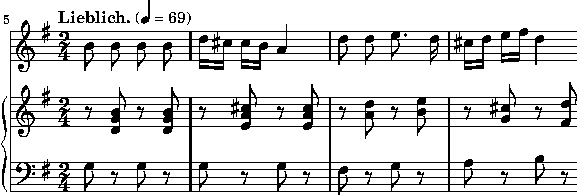
\includegraphics{documentation/example-document/single-system-example.preview.pdf}
  \caption{My first music example}
\end{musicExample}
\end{document}
\end{verbatim}

If that compiles without errors you have successfully installed \package{musicexamples}.



\section{musicexamples.sty}
\label{sec:xmp_musicexamples}

\texttt{musicexamples} is a \LaTeX{} package that defines environments and commands to handle music examples (scores and fragments) within \LaTeX{} documents.
It supports floating or non-floating examples as well as full-(one- or multi-)page scores.
The examples are numbered in one contigious list and can be output as one \cmd{listofmusicexamples}, regardless of their type of inclusion.

The package was developed from the perspective of a user of the LilyPond notation software%
\footnote{\url{http://www.lilypond.org}}, but you can use it with any kind of suitable music example images.
The package has some similarities with LilyPond's \package{lilypond-book} script, but it doesn't understand itself as a competitor for this, but rather as a different approach for people with somewhat different needs.
It can even be used in parallel, i.\,e.\ you can use \package{musicexamples'} environments to wrap \package{lilypond-book}-like source snippets.
For anybody writing (about) music it may also be a good idea to have a look at my \package{lilyglyphs} package that is \package{musicexample}s sibling in the \package{openLilyLib} family of resources.

The following documentation is split into “basic” and “advanced” usage sections because there are basic possibilities that you can use without bothering about the advanced ones.
Especially you are in no way forced to use LilyPond as the source of your music examples (although I can't recommend it highly enough \dots).
In the basic “mode” you can simply use \package{musicexamples} as a tool to number and list your music examples.

\subsection{Basic Usage}
\label{subsec:xmp_basic-usage}
In order to use \texttt{musicexamples} you simply \emph{use} or \emph{Require} the \package\{musicexamples\} 
in your document preamble.
You will then have access to its commands and environments.

Music examples printed by any of the following environments or commands are numbered in one list (they share the counter \env{musicexamples}).
You can create a list of music examples just as you would create a list of tables or figures with the command \cmd{listofmusicexamples}.
The list title defaults to “List of Music Examples” and can be changed using \cmd{setXmpListName}.


\subsubsection{Environments for Shorter Music Examples}
\label{subsubsec:xmp_basic-usage_environments}

There are two environments to be used for non-fullpage music examples: \env{musicExample} and \env{musicExampleNonFloat}.
The point of having a non-floating environment to \emph{not} to have more control over the placement of the item, but rather to allow it to cross page breaks, so that a group of music systems may flow over one or more pages. 
These environments do not print the music examples themselves but only provide the environment for them (as a \texttt{figure} environment doesn't already print the figure), managing their placement, captions, numbering and listing.

You use \env{musicExample} like any other float environment, so you can optionally add the placement directive after the \cmd{begin} statement (of the floating version).
Inside the environment you add the contents, the \cmd{caption} to be used, and a \cmd{label}.
\begin{quote}
\begin{verbatim}
% Usage example
\begin{musicExample}[t]
  \includegraphics{exampleimage}
  \caption{A typical music example}
  \label{xmp:typical-example}
\end{musicExample}
\end{verbatim}
\end{quote}

This will print your image in a floating environment [preferrably at the top of a page], will take care of the numbering and prepares for the inclusion in a list of music examples.
\package{musicexamples} loads the \package{fancyref} package, and you can profit from the predefined set of reference strings for the new \texttt{xmp:} prefix shown in the example.
There are also German strings provided if you load \package{fancyref} with the \texttt{german} option, but this doesn't work yet \ghIssue{7} \todo{Look for the right issue}.

The usage of \env{musicExampleNonFloat} is identical, except that it doesn't accept the optional placement argument.
It will print the example right where you inserted the environment, and while the floating version can only print the example in a box on a single page, this one can spread over page breaks -- provided the music systems are given as separate images.

The captions are standard captions that can be formatted with the commands of the \package{caption} package (please refer to its documentation).
The caption label defaults to “Music Example” but you can change this with the command \cmd{setXmpCaptionLabel} with one mandatory argument supplying the desired string.
The alignment of the caption is centered by default, but you can of course change this behaviour, either locally or generally:
To change a single example you can just enter an alignment command (like \cmd{flushleft} or \cmd{flushright}) inside the environment, just before the image.
To change the behaviour of all subsequent floating or non-floating environments you may use the \cmd{setXmpAlignment} command with the appropriate command as its argument.

\begin{quote}
\begin{verbatim}
% Change the labelname of subsequent captions
\setXmpCaptionLabel{Notenbeispiel}

% Change alignment of subsequent music examples
\setXmpAlignment{\flushleft}

% Change the alignment of the current music example
\begin{musicExample}
  \flushright
  \includegraphics{exampleimage}
\end{musicExample}
\end{verbatim}
\end{quote}

The \package{newfloat} package that was used to define the new floating environment offers a nice feature:
If you have loaded certain other packages it will automagically create some other commands of floating environments for you.
They behave the same as their standard counterparts, and for further information please refer to the respective package documentation.

\begin{description}
\item[\cmd{wrapmusicexample}] is created by loading the \texttt{wrapfig} package.
It will create a floating music example that is wrapped by the continuous text.
\item[\cmd{sidewaysmusicexample}] is created by loading the \texttt{rotating} package.
It will create a music example that is rotated so you can use examples with a landscape page layout.
\item[\cmd{SCmusicexample}] is created by loading the \texttt{sidecap} package.
It will create a music example with the caption placed beside.
\item[{\cmd{FPmusicexample}}] is created by loading the \texttt{fltpage} package.
It will create a music example with the caption placed on the previous or next page.
As \texttt{musicexamples} offers its own solution for full-page music examples (see below) you probably won't need this.
\end{description}

\subsubsection{Full Page Music Examples}
\label{subsubsec:xmp_basic-usage_full-page-examples}

The \cmd{fullPageMusicExample} command gives you the possibility to include pdf files as full-page scores with one or more pages.
It behaves differently from the above \emph{environments} in that it is a \emph{command} -- and in that it actually inserts the example in the document instead of only providing its environment.
The command expects three mandatory arguments: 
\# 1: the file name (including the relative path but without the extension) to a pdf (and no other image) file,
\#2: the caption and \#3: a \cmd{label} command.
While it would have been easy to let you provide only the label itself, it makes sense to use this somewhat redundant syntax.
This way you actually have a \cmd{label} at the right place in your source which your editor may use to help you navigate your document.

\begin{quote}
\begin{verbatim}
% Usage example
\fullPageMusicExample
    {examples/chapter01/helpfulexample} % path to image
    {A helpful example} % caption text
    {\label{xmp:helpful-example}}
\end{verbatim}
\end{quote}
Internally the pages are included using \cmd{includepdf} and the \package{afterpage} package, so the score will start at the next page without leaving the rest of the current page empty.
The label will be placed correctly on the new page so references will be correct.
Great effort has been put into the handling of examples starting on odd or even pages (see below for details).

The handling of the caption is somewhat special with this command.
The caption -- which isn't a real \cmd{caption} but just text used as such -- is printed in the header or footer of the (first) page of the example.
This is realized through the use of the \package{scrpage2} package from \package{KOMA-Script}.
The pagestyle for the first page is set to the predefined \env{xmpPageOne} while the remaining pages are assigned \env{xmpPageTwo}.
By default the caption is printed on the left (or inner) part of the header of the first page, while the page number is centered in the footer.
The caption is styled manually within this page style and defaults to the default \cmd{caption} format.
If you want to adapt these formats (page layout or caption formatting) you will have to redefine one or both formats using \cmd{deftripstyle} (see the KOMA-Script documentation for details).
Note that if you change the formatting of the captions using \cmd{captionsetup} you will have to adjust these page styles too.
Take the definition of the styles in the package as an example.
The first argument is the name of the style to be modified, the next three arguments take what is to be printed in the three parts of the header, and finally there are three arguments for the footer.
\begin{quote}
\begin{verbatim}
% Example of changing the page styles for full page examples
\deftripstyle{xmpPageOne}%
{\upshape\ollXmpCaptionLabel \arabic{musicexample}: \xmpCaption}{}{}%
{}{--\,\pagemark\,--}{}

\deftripstyle{xmpPageTwo}%
{}{}{}
{}{--\,\pagemark\,--}{}

\end{verbatim}
\end{quote}

The full-page example command first checks if there is a pdf file on disk with the basename given as the first argument or with one of the suffixes \texttt{-odd} or \texttt{-even}.
If none of them is present there will be a colored box indicating the missing full-page example, additionally the entry in the list of music examples (if you have one) will be colored red.
The message in the box defaults to “Missing full-page example:“, but you can configure it with \cmd{setXmpMissingFullpageLabel}.

Through the use of file name suffixes you can control the placement of your full-page music examples.
Files with the plain name are considered as one-sided, i.\,e.\ as being able to start at an arbitrary page. 
File names with a suffix indicate two-sided layout with the first page being odd or even respectively.
If you have a score with one-sided layout then you will provide just the file with the plain basename, and it will be printed starting at the next page.
If you have a score with two-sided layout but you don't mind it starting on an odd or even page you should provide two files with both suffixes, the command will then print the example starting on the next page and use the appropriate example file.
If you finally have a two-sided score that should explicitely start on an odd or even page (typically one might want to have two page scores printed on one double page for example) then you should only provide one file with the appropriate suffix, which will be printed on the next odd or even page (as indicated by the file suffix), possibly skipping another page of text.

\medskip
\cmd{fullPageLilypondExample} behaves the same as \cmd{fullPageMusicExample} but you should use it for examples created with LilyPond, as it can be used (e.\,g.\ by scripts) to keep track of these examples (see \fref{chap:xmp_python}).

\begin{knownIssues}
The LilyPond configuration files provide functions to compile odd- and even-starting pdf files from one source file, but they are not quite perfect and not documented yet. 
Maybe I'll also implement the possibility to include “cropped“ scores (without page margins) that can be scaled into the text area of the \LaTeX{} document.
And maybe I'll implement functionality to use one-sided scores (on smaller paper) that are placed correctly on the page (but that's only an idea so far).
\end{knownIssues}

\bigskip

\subsection{Advanced Usage}
\label{subsec:xmp_advanced-usage}

So far we have discussed the environments to place music examples in and the commands to print full-page examples.
Now we're going to see how to actually print music examples inside the environments.

You are free to enter anything (presumably images) within the environments and use them as a kind of specific \env{figure} environment (as was shown in the first example).
But we have provided several commands that are explicitely intended for printing the music examples which give you a consistent interface and perhaps a few other advantages.

\cmd{musicSFE} and \cmd{lilypondSFE} are used to print Single File Examples.
Technically they print one \emph{file}, but for the sake of consistency it is recommended to use them for examples with one \emph{music system} only.

As with the full-page examples the “lilypond” versions is technically the same as the “music” version, but you should use them to distinguish between music examples provided by arbitrary image files and examples generated by LilyPond.
\\\todo{Note: The script hasn't been implemented yet.}

You use both commands by providing the file basename as the mandatory argument, including the relative path but excluding the extension.
Internally these commands include the example with \cmd{includegraphics}, and you can pass an optional argument with the same options that you can use to include images normally.
However it is usually recommendable to prepare the images with the right size in advance and include them unaltered in order to get a consistent layout.
\package{musicexamples} uses the \package{adjustbox} package which extends the capabilities of \package{graphicx} and adds some keys to it that you can also use (see the package documentation).

The image is included in its own paragraph without indentation, and it is centered by default.
If you provide an image with a width of \cmd{textwidth} the example will fill the whole line.
If the width of the image is smaller then it will be centered by default, and if it exceeds the text width it will automatically be scaled to the text width.
So images will never protrude out of the text area, but you have to expect resizing if you provide too large images.
You can override the alignment manually with standard LaTeX commands inside the environment, or you can set the alignment for all subsequent musicexamples with \cmd{setXmpAlignment\{alignment-command\}} (both as demonstrated before).

If you provide a filename that doesn't point to an existing and valid image file two things will happen:
Instead of giving and error message to the log file the command will print a colored box with a message in it, and the caption will be colored red in the list of musicexamples (if you have one).
The point of this isn't mainly to spot missing image files, but rather to be able to safely enter placeholders for music examples that haven't yet been created.
The message in the box defaults to “Missing Image:“, but you can configure it with \cmd{setXmpMissingImageLabel}.
I didn't bother to make the appearance of the box configurable so far because I regard this as a convenience tool for document authors that shouldn't be part of a final version.
But feel free to suggest improvements.
You can use file names with more than one dot in it (like the default output files of LilyPond with the \texttt{-dpreview} option). 
In this case you still leave out the \texttt{.pdf} part but enclose the file name in \emph{three} pairs of curly braces, like \cmd{musicSFE\{\{\{example-image.preview\}\}\}}.

\begin{knownIssues}
You shouldn't actually use special characters in file names.
While \cmd{includegraphics} may handle some of them, the other functions probably won't. 
If your filename contains underscores for example the image will be printed just fine, but if the image is missing, \LaTeX{} will try to print the filename -- which it can't because of the underscore -- which will result in strange error messages.
\end{knownIssues}

\begin{quote}
\begin{verbatim}
% Use of the printing command together with the optional argument
\lilypondSFE[scale=1.2]{examples/lilypond/example1}
\end{verbatim}
\end{quote}

\cmd{lilypondMFE} is used to print a Multi File Example generated by LilyPond.
With this kind of examples the difference between \env{musicExample} and \env{musicExampleNonFloat} becomes important.
The floating environment can only print the example onto a single page, so you will want to use it if the example won't exceed a page, and you want to keep it together.
The non-floating variant is useful if you want the example to flow naturally with the text and allow it to be laid out across page breaks.

There is no “music“ variant of this command because it expects a series of music systems in a form that is typical for LilyPond's \texttt{lilypond-book} style output.
(We will discuss some aspects on how to streamline the creation of these examples on the LilyPond side in \fref{chap:xmp_lilypond-configuration}).
If you have a music example consisting of several individual image files you can still use \cmd{musicSFE} multiple times to print them manually.

To use \cmd{lilypondMFE} you provide the file basename as the mandatory argument, just like with the other commands we saw so far.
As with \cmd{lilypondSFE} this command accepts an optional argument and passes it unchanged to \cmd{includegraphics}.
To work correctly the command expects a set of files to be present at the location specified by the argument.
These are some of the files that you'll find when you include the file \texttt{lilypond-book-preamble.ly} in your LilyPond document:
\begin{description}
\item[\texttt{BASENAME-\#(.pdf)}] Numbered files for each system.
The music systems start with \#\,3, while the first two files are the book and score title markups, which are discarded by the command
\item[\texttt{BASENAME-systems.count}] is a file containing exclusively one number indicating the number of systems to be processed.
This number includes the first two unused systems, so if you have an example with three systems this file will actually contain the number 5.
\end{description}

\cmd{lilypondMFE} will now iterate over the files 3 to n to consecutively print the systems using the \cmd{musicSFE} command.
\\\todo{It is intended to implement some optional element between consecutive systems (just as  \texttt{lilypond-book} does) \ghIssue{6}.}

As mentioned the book and score title markups from the LilyPond score are discarded by this command.
If you need to have titles in the example you will have to supply them directly within the music example environment or as markups in the LilyPond score (not in the header but in the music part).

\subsection{Command Reference}
\label{subsec:xmp_command-reference}
To finish off this section I will provide a short list of the available commands:

\subsubsection*{Environments to Place Music Examples in}
\label{subsubsec:environments}
\begin{description}
\item[\env{musicExample}] Floating environment, content is centered by default.
\item[\env{musicExampleNonFloat}] Non-floating environment that can enclose multiple images across page breaks.
\end{description}

More optional floating environments that are available when third-party packages are loaded (some comments earlier in \fref{sec:xmp_basic-usage}, more information in the respective package documentation):
\begin{description}
\item[\cmd{wrapmusicexample}](\texttt{wrapfig})
\item[\cmd{sidewaysmusicexample}] (\texttt{rotating})
\item[\cmd{SCmusicexample}] (\texttt{sidecap})
\item[{\cmd{FPmusicexample}}] (\texttt{fltpage})
\end{description}

\subsection*{Commands that Print Music Examples}
\begin{description}
\item[\cmd{musicSFE} and \cmd{lilypondSFE}]Print a single file (system).
\item[\cmd{lilypondMFE}]Print a music example consisting of several files.
\item[\cmd{fullPageMusicExample}] \emph{Command} that prints full-page music examples.
Starting examples on odd or even pages is fully supported.
\item[\cmd{fullPageLilypondExample}] Same as above, but to be used for LilyPond generated examples.
\end{description}

\subsection*{Miscellaneous Options and Commands}
\begin{description}
\item[\cmd{SetupFloatingEnvironment}](\package{caption}): Modify the appearance of the captions of the (floating and non-floating) environments.
\item[\cmd{setXmpCaptionLabel}]Set the label used for the captions (e.\,g.\ set it to your own language)
\item[\cmd{setXmpListName}]Set the Title for the list of music examples.
\item[\cmd{setXmpAlignment}] Set the alignment for all subsequent music examples.
To modify the alignment of a single example use standard \LaTeX{} commands inside the environment.
\item[\env{xmpPageOne} and \env{xmpPageTwo}]Page styles used (by \package{scrpage2}) for the first and the remaining pages of a full/multi page example. 
Typically prints the caption in the header or footer of the first page.
The caption has to be manually made consistent with the standard captions.
To change the layout use the \cmd{deftripstyle} command from the \package{scrpage2} package.
\item[\env{\{xmp:\}}] Suggested prefix for labels.
There are \package{fancyref} labels defined for this prefix.
\end{description} 

\section{Using \env{musicexamples} with Plain LilyPond}
\label{sec:xmp_lilypond}

Although it is not really recommended \env{musicexamples} works well with scores
generated by LilyPond separately. Basically the package will treat such scores
agnostically as image files, and it's the responsibility of the author of the
LilyPond files to make them work smoothly with the text document. However, it
may be necessary to go that route when it is not possible to use the
\package{lyluatex} package with \LuaLaTeX\ as explained in the next chapter. The most important caveats are:

\begin{itemize}
\item Staff size and line width have to be set explicitly to match the
appearance of the final text document. The tools don't give any support for
adjusting the scores to changes in the document layout.

\item Full-page scores also have to make sure their page margins match that of
the text document. Specific care has to be taken with two-sided layout.
\package{musicexamples} is able to detect the presence of an \texttt{-odd} or
\texttt{-even} suffix to the file name to automatically start the score on an
odd or even page. But it is completely up to the author of the LilyPond files to
ensure correct behaviour.

\item Full-page scores should generally suppress the printing of headers and
footers, and leave this to \LaTeX. This is especially useful for pagination
purposes.

\item When printing the caption in the header of full-page scores some extra
top-margin should be left in the scores.

\item \emph{One system examples} should be compiled with LilyPond's “preview”
option, which causes the output file to be cropped to its minimal dimension.

\item For \emph{multi system examples} you should 
\verb+\include "lilypond-book-preamble.ly"+ somewhere in your document. 
This lets LilyPond output each system as a separate (cropped) file with
a naming convention that allows \package{musicexample}'s \cmd{lilypondMFE}
command to iterate over all systems to print them.
\end{itemize}

\section{Using \package{musicexamples} with \package{lyluatex}}
\label{sec:xmp_lyluatex}

\package{musicexamples} is designed to work well with the \package{lyluatex} package.\footnote{\url{https://ctan.org/pkg/lyluatex}}

\todo{To be documented}

\end{document}